\documentclass[aspectratio=169]{beamer}
\usetheme{Madrid}
\usecolortheme{whale}

\usepackage{graphicx}
\usepackage{listings}
\usepackage{xcolor}
\usepackage{tikz}
\usetikzlibrary{shapes,arrows,positioning,calc}
\usepackage{booktabs}
\usepackage{adjustbox}

% Code listing style - escape special chars
\lstset{
    basicstyle=\ttfamily\tiny,
    keywordstyle=\color{blue},
    commentstyle=\color{gray},
    stringstyle=\color{orange},
    breaklines=true,
    frame=single,
    backgroundcolor=\color{gray!10},
    escapeinside={(*@}{@*)},
    literate={\_}{\_}1
}

\title{Hotel Recommendation Chatbot}
\subtitle{Graph-Based RAG System with Multi-Model Integration}
\author{Team Name}
\date{\today}

\begin{document}

%==============================================================================
\begin{frame}
\titlepage
\end{frame}

%==============================================================================
% SECTION 1: HIGH-LEVEL SYSTEM ARCHITECTURE
%==============================================================================
\section{System Architecture}

\begin{frame}{System Architecture Overview}
\begin{center}
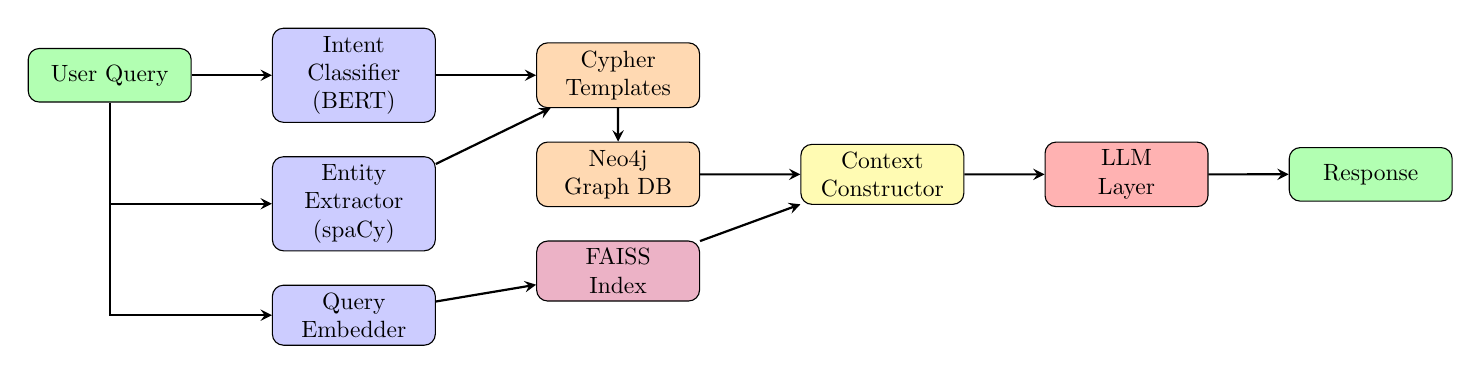
\begin{tikzpicture}[node distance=1.2cm, scale=0.85, transform shape,
    block/.style={rectangle, draw, fill=blue!20, text width=2.2cm, text centered, minimum height=0.8cm, rounded corners},
    arrow/.style={->, >=stealth, thick}]

    % Input
    \node[block, fill=green!30] (input) {User Query};

    % Preprocessing
    \node[block, right=of input] (intent) {Intent\\Classifier\\(BERT)};
    \node[block, below=0.5cm of intent] (entity) {Entity\\Extractor\\(spaCy)};
    \node[block, below=0.5cm of entity] (embed) {Query\\Embedder};

    % Retrieval
    \node[block, right=1.5cm of intent, fill=orange!30] (cypher) {Cypher\\Templates};
    \node[block, below=0.5cm of cypher, fill=orange!30] (neo4j) {Neo4j\\Graph DB};
    \node[block, below=0.5cm of neo4j, fill=purple!30] (faiss) {FAISS\\Index};

    % Context
    \node[block, right=1.5cm of neo4j, fill=yellow!30] (context) {Context\\Constructor};

    % LLM
    \node[block, right=of context, fill=red!30] (llm) {LLM\\Layer};

    % Output
    \node[block, right=of llm, fill=green!30] (output) {Response};

    % Arrows
    \draw[arrow] (input) -- (intent);
    \draw[arrow] (input) |- (entity);
    \draw[arrow] (input) |- (embed);
    \draw[arrow] (intent) -- (cypher);
    \draw[arrow] (entity) -- (cypher);
    \draw[arrow] (cypher) -- (neo4j);
    \draw[arrow] (embed) -- (faiss);
    \draw[arrow] (neo4j) -- (context);
    \draw[arrow] (faiss) -- (context);
    \draw[arrow] (context) -- (llm);
    \draw[arrow] (llm) -- (output);

\end{tikzpicture}
\end{center}

\vspace{0.3cm}
\textbf{Task:} Hotel Recommendation Chatbot with visa-aware travel suggestions

\textbf{Dataset:} Custom hotel reviews dataset (hotels, users, reviews, visa requirements)
\end{frame}

%==============================================================================
% SECTION 2: INPUT PREPROCESSING
%==============================================================================
\section{Input Preprocessing}

\begin{frame}{Intent Classification - BERT Fine-tuned}
\begin{columns}
\begin{column}{0.5\textwidth}
\textbf{Model:} \texttt{bert-base-uncased}

\textbf{Training Config:}
\begin{itemize}
    \item Learning rate: 5e-5
    \item Batch size: 16
    \item Epochs: 15
    \item Train/Test split: 85/15
\end{itemize}

\vspace{0.3cm}
\textbf{10 Intent Classes:}
\begin{enumerate}
    \scriptsize
    \item hotel\_recommendation
    \item hotel\_search
    \item hotel\_info
    \item review\_query
    \item comparison
    \item traveller\_preference
    \item location\_query
    \item visa\_query
    \item rating\_filter
    \item general\_question
\end{enumerate}
\end{column}

\begin{column}{0.5\textwidth}
\textbf{Classification Examples:}

\vspace{0.2cm}
\begin{tabular}{|p{4cm}|l|}
\hline
\textbf{Query} & \textbf{Intent} \\
\hline
``Recommend me a hotel in Tokyo'' & hotel\_rec (0.97) \\
\hline
``Do I need visa from India?'' & visa\_query (0.89) \\
\hline
``Compare Azure Tower and Marina'' & comparison (0.94) \\
\hline
``Best for business travelers'' & traveller\_pref (0.91) \\
\hline
``Hotels with rating above 9'' & rating\_filter (0.88) \\
\hline
\end{tabular}
\end{column}
\end{columns}
\end{frame}

%------------------------------------------------------------------------------
\begin{frame}{Entity Extraction - spaCy + Custom Rules}
\begin{columns}
\begin{column}{0.45\textwidth}
\textbf{Approach:} Hybrid (NER + Token Matching)

\vspace{0.2cm}
\textbf{Entity Types Extracted:}
\begin{itemize}
    \item \textbf{Hotels} - FAC, ORG labels + lookup
    \item \textbf{Cities/Countries} - GPE label
    \item \textbf{Traveller Types} - Token matching
    \item \textbf{Demographics} - Gender, Age groups
    \item \textbf{Ratings} - Cleanliness, Comfort, Facilities
\end{itemize}

\vspace{0.2cm}
\textbf{Traveller Keywords:}
\begin{itemize}
    \scriptsize
    \item solo, alone $\rightarrow$ ``Solo''
    \item business, corporate $\rightarrow$ ``Business''
    \item family, families $\rightarrow$ ``Family''
    \item couple, couples $\rightarrow$ ``Couple''
\end{itemize}
\end{column}

\begin{column}{0.55\textwidth}
\textbf{Extraction Examples:}

\vspace{0.2cm}
\footnotesize
\texttt{Query: ``Best hotels for solo female in Paris''}
\begin{itemize}
    \scriptsize
    \item cities: [``Paris'']
    \item traveller\_types: [``Solo'']
    \item demographics: [``Female'']
\end{itemize}

\vspace{0.2cm}
\texttt{Query: ``Hotels with cleanliness above 9''}
\begin{itemize}
    \scriptsize
    \item cleanliness\_base: 9.0
    \item comfort\_base: None
    \item facilities\_base: None
\end{itemize}

\vspace{0.2cm}
\texttt{Query: ``Compare Azure Tower and Marina Bay''}
\begin{itemize}
    \scriptsize
    \item hotels: [``The Azure Tower'', ``Marina Bay'']
\end{itemize}
\end{column}
\end{columns}
\end{frame}

%------------------------------------------------------------------------------
\begin{frame}{Query Embedding}
\begin{columns}
\begin{column}{0.5\textwidth}
\textbf{Model:} \texttt{all-MiniLM-L6-v2}

\textbf{Properties:}
\begin{itemize}
    \item Embedding dimension: 384
    \item Optimized for semantic similarity
    \item Used for both query and hotel embeddings
\end{itemize}

\vspace{0.3cm}
\textbf{Code Snippet:}

\footnotesize
\texttt{from sentence\_transformers import SentenceTransformer}

\texttt{model = SentenceTransformer('all-MiniLM-L6-v2')}

\texttt{def embed\_query(text):}

\texttt{~~~~return model.encode(text)}
\end{column}

\begin{column}{0.5\textwidth}
\textbf{Usage in Pipeline:}
\begin{enumerate}
    \item User query $\rightarrow$ 384-dim vector
    \item FAISS similarity search
    \item Retrieve semantically similar hotels
    \item Combine with Cypher results
\end{enumerate}

\vspace{0.3cm}
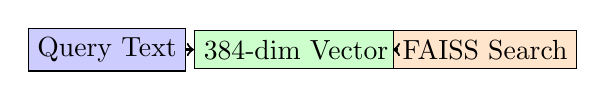
\begin{tikzpicture}[scale=0.8]
    \node[draw, rectangle, fill=blue!20] (q) at (0,0) {Query Text};
    \node[draw, rectangle, fill=green!20] (e) at (3,0) {384-dim Vector};
    \node[draw, rectangle, fill=orange!20] (f) at (6,0) {FAISS Search};
    \draw[->, thick] (q) -- (e);
    \draw[->, thick] (e) -- (f);
\end{tikzpicture}
\end{column}
\end{columns}
\end{frame}

%==============================================================================
% SECTION 3: GRAPH RETRIEVAL - BASELINE
%==============================================================================
\section{Graph Retrieval - Baseline}

\begin{frame}{Knowledge Graph Schema}
\begin{center}
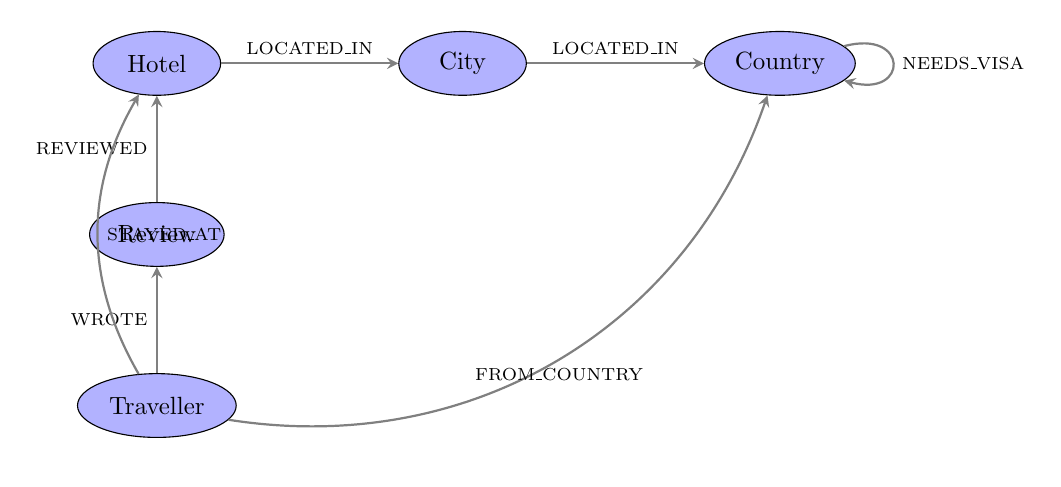
\begin{tikzpicture}[node distance=2cm, scale=0.9, transform shape,
    entity/.style={ellipse, draw, fill=blue!30, minimum width=1.8cm, minimum height=0.9cm},
    rel/.style={->, >=stealth, thick, draw=gray}]

    % Nodes
    \node[entity] (hotel) {Hotel};
    \node[entity, right=2.5cm of hotel] (city) {City};
    \node[entity, right=2.5cm of city] (country) {Country};
    \node[entity, below=1.5cm of hotel] (review) {Review};
    \node[entity, below=1.5cm of review] (traveller) {Traveller};

    % Relationships
    \draw[rel] (hotel) -- node[above, font=\scriptsize] {LOCATED\_IN} (city);
    \draw[rel] (city) -- node[above, font=\scriptsize] {LOCATED\_IN} (country);
    \draw[rel] (review) -- node[left, font=\scriptsize] {REVIEWED} (hotel);
    \draw[rel] (traveller) -- node[left, font=\scriptsize] {WROTE} (review);
    \draw[rel] (traveller) to[bend left=30] node[right, font=\scriptsize] {STAYED\_AT} (hotel);
    \draw[rel] (traveller) to[bend right=40] node[below, font=\scriptsize] {FROM\_COUNTRY} (country);
    \draw[rel] (country) to[loop right, looseness=5] node[right, font=\scriptsize] {NEEDS\_VISA} (country);

\end{tikzpicture}
\end{center}

\vspace{0.3cm}
\begin{columns}
\begin{column}{0.5\textwidth}
\textbf{Node Properties:}
\begin{itemize}
    \scriptsize
    \item Hotel: name, star\_rating, cleanliness, comfort, facilities
    \item Review: text, date, scores (overall, cleanliness, etc.)
    \item Traveller: age, gender, type
\end{itemize}
\end{column}
\begin{column}{0.5\textwidth}
\textbf{Relationships (7 types):}
\begin{itemize}
    \scriptsize
    \item LOCATED\_IN, REVIEWED, WROTE
    \item FROM\_COUNTRY, STAYED\_AT
    \item NEEDS\_VISA (with visa\_type property)
\end{itemize}
\end{column}
\end{columns}
\end{frame}

%------------------------------------------------------------------------------
\begin{frame}{Cypher Query Templates (1/2)}
\begin{columns}
\begin{column}{0.5\textwidth}
\textbf{Location Queries:}
\footnotesize

\vspace{0.1cm}
\texttt{-- Hotels in city}

\texttt{MATCH (h:Hotel)-[:LOCATED\_IN]->(c:City)}

\texttt{WHERE c.name = \$city}

\texttt{RETURN h.name, h.star\_rating}

\vspace{0.2cm}
\texttt{-- Top rated in country}

\texttt{MATCH (h:Hotel)-[:LOCATED\_IN]->(c:City)}

\texttt{~~~~~~-[:LOCATED\_IN]->(co:Country)}

\texttt{WHERE co.name = \$country}

\texttt{RETURN h.name ORDER BY h.star\_rating DESC}

\vspace{0.2cm}
\texttt{-- Cities with hotels}

\texttt{MATCH (h:Hotel)-[:LOCATED\_IN]->(c:City)}

\texttt{RETURN DISTINCT c.name, h.name}
\end{column}

\begin{column}{0.5\textwidth}
\textbf{Review Queries:}
\footnotesize

\vspace{0.1cm}
\texttt{-- Hotel reviews}

\texttt{MATCH (h:Hotel)<-[:REVIEWED]-(r:Review)}

\texttt{WHERE h.name = \$hotel\_name}

\texttt{RETURN r.text, r.score\_overall LIMIT 10}

\vspace{0.2cm}
\texttt{-- Reviews by demographic}

\texttt{MATCH (h:Hotel)<-[:REVIEWED]-(r:Review)}

\texttt{~~~~~~<-[:WROTE]-(t:Traveller)}

\texttt{WHERE h.name = \$hotel\_name}

\texttt{~~AND t.gender = \$gender}

\texttt{RETURN r.text, r.score\_overall}
\end{column}
\end{columns}
\end{frame}

%------------------------------------------------------------------------------
\begin{frame}{Cypher Query Templates (2/2)}
\begin{columns}
\begin{column}{0.5\textwidth}
\textbf{Visa \& Traveller Queries:}
\footnotesize

\vspace{0.1cm}
\texttt{-- Countries requiring visa}

\texttt{MATCH (tc:Country)-[:NEEDS\_VISA]->(co:Country)}

\texttt{WHERE tc.name = \$from\_country}

\texttt{RETURN co.name}

\vspace{0.2cm}
\texttt{-- Hotels without visa needed}

\texttt{MATCH (tc:Country), (h:Hotel)-[:LOCATED\_IN]}

\texttt{~~~~~~->(c:City)-[:LOCATED\_IN]->(co:Country)}

\texttt{WHERE tc.name = \$from AND NOT}

\texttt{~~~~~~(tc)-[:NEEDS\_VISA]->(co)}

\texttt{RETURN DISTINCT h.name}

\vspace{0.2cm}
\texttt{-- Best for traveller type}

\texttt{MATCH (h:Hotel)<-[:REVIEWED]-(r:Review)}

\texttt{~~~~~~<-[:WROTE]-(t:Traveller)}

\texttt{WHERE t.type = \$type}

\texttt{RETURN h.name, AVG(r.score\_overall)}
\end{column}

\begin{column}{0.5\textwidth}
\textbf{Rating \& Comparison:}
\footnotesize

\vspace{0.1cm}
\texttt{-- Hotels by cleanliness}

\texttt{MATCH (h:Hotel)}

\texttt{WHERE h.cleanliness\_base >= \$min}

\texttt{RETURN h.name, h.cleanliness\_base}

\texttt{ORDER BY h.cleanliness\_base DESC}

\vspace{0.2cm}
\texttt{-- Compare two hotels}

\texttt{MATCH (h1:Hotel), (h2:Hotel)}

\texttt{WHERE h1.name = \$hotel1}

\texttt{~~AND h2.name = \$hotel2}

\texttt{RETURN h1, h2}

\vspace{0.2cm}
\texttt{-- Hotels with most reviews}

\texttt{MATCH (h:Hotel)<-[:REVIEWED]-(r:Review)}

\texttt{RETURN h.name, COUNT(r) as cnt}

\texttt{ORDER BY cnt DESC LIMIT \$top\_n}

\vspace{0.3cm}
\textbf{Total: 31 Cypher Templates}
\end{column}
\end{columns}
\end{frame}

%------------------------------------------------------------------------------
\begin{frame}{Retrieved Data Examples}
\textbf{Query:} ``Recommend me a hotel in Tokyo''

\begin{columns}
\begin{column}{0.5\textwidth}
\textbf{Pipeline Output:}
\begin{itemize}
    \item Intent: hotel\_recommendation
    \item Entities: cities=[``Tokyo''], countries=[``Japan'']
\end{itemize}

\vspace{0.2cm}
\textbf{Cypher Results:}

\footnotesize
\begin{tabular}{|l|c|l|}
\hline
\textbf{Hotel} & \textbf{Rating} & \textbf{City} \\
\hline
The Azure Tower & 4.8 & Tokyo \\
Sakura Grand Hotel & 4.6 & Tokyo \\
Imperial Garden Inn & 4.5 & Tokyo \\
\hline
\end{tabular}
\end{column}

\begin{column}{0.5\textwidth}
\textbf{Query:} ``Best for business travelers''

\vspace{0.2cm}
\textbf{Pipeline Output:}
\begin{itemize}
    \item Intent: traveller\_preference
    \item Entities: traveller\_types=[``Business'']
\end{itemize}

\vspace{0.2cm}
\textbf{Cypher Results:}

\footnotesize
\begin{tabular}{|l|c|}
\hline
\textbf{Hotel} & \textbf{Avg Score} \\
\hline
Executive Suites & 9.2 \\
Business Bay Hotel & 8.9 \\
Corporate Tower & 8.7 \\
\hline
\end{tabular}
\end{column}
\end{columns}
\end{frame}

%==============================================================================
% SECTION 4: EMBEDDING-BASED RETRIEVAL
%==============================================================================
\section{Embedding-Based Retrieval}

\begin{frame}{Dual Embedding Approach}
\begin{center}
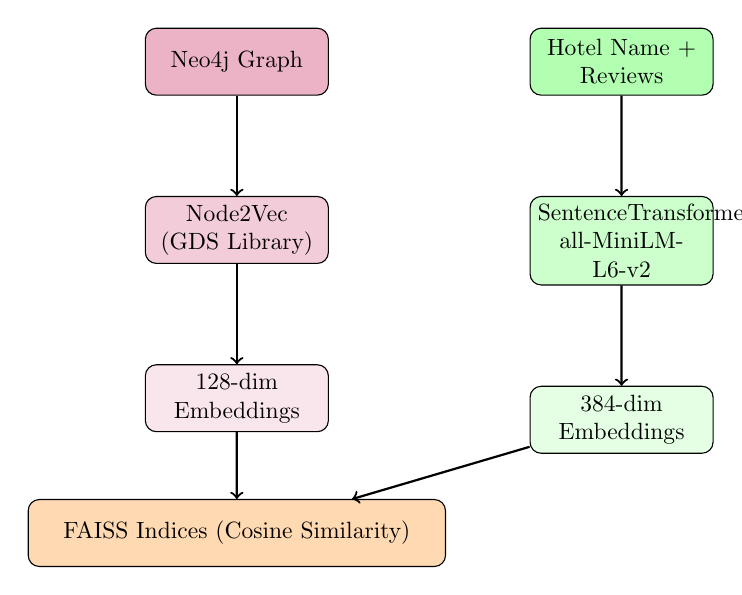
\begin{tikzpicture}[node distance=1.5cm, scale=0.85, transform shape,
    block/.style={rectangle, draw, fill=blue!20, text width=2.5cm, text centered, minimum height=1cm, rounded corners}]

    % Left side - Node2Vec
    \node[block, fill=purple!30] (graph) {Neo4j Graph};
    \node[block, below=of graph, fill=purple!20] (n2v) {Node2Vec\\(GDS Library)};
    \node[block, below=of n2v, fill=purple!10] (n2vemb) {128-dim\\Embeddings};

    % Right side - Text
    \node[block, right=3cm of graph, fill=green!30] (text) {Hotel Name +\\Reviews};
    \node[block, below=of text, fill=green!20] (st) {SentenceTransformer\\all-MiniLM-L6-v2};
    \node[block, below=of st, fill=green!10] (stemb) {384-dim\\Embeddings};

    % FAISS
    \node[block, below=1cm of n2vemb, fill=orange!30, text width=6cm] (faiss) {FAISS Indices (Cosine Similarity)};

    % Arrows
    \draw[->, thick] (graph) -- (n2v);
    \draw[->, thick] (n2v) -- (n2vemb);
    \draw[->, thick] (text) -- (st);
    \draw[->, thick] (st) -- (stemb);
    \draw[->, thick] (n2vemb) -- (faiss);
    \draw[->, thick] (stemb) -- (faiss);

\end{tikzpicture}
\end{center}

\vspace{0.3cm}
\textbf{Selected Approach:} Feature Vector Embeddings (Text + Graph Structure)
\end{frame}

%------------------------------------------------------------------------------
\begin{frame}{Embedding Models Comparison}
\begin{table}
\centering
\begin{tabular}{lcc}
\toprule
\textbf{Property} & \textbf{Node2Vec} & \textbf{Text Embeddings} \\
\midrule
Model & GDS Node2Vec & all-MiniLM-L6-v2 \\
Dimension & 128 & 384 \\
Input & Graph structure & Hotel name + reviews \\
Captures & Relationships, paths & Semantic meaning \\
\midrule
Walk Length & 40 & -- \\
Iterations & 10 & -- \\
Buffer Size & 1000 & Batch size: 32 \\
\bottomrule
\end{tabular}
\caption{Embedding Configuration Comparison}
\end{table}

\vspace{0.3cm}
\begin{columns}
\begin{column}{0.5\textwidth}
\textbf{Node2Vec Strengths:}
\begin{itemize}
    \item Captures hotel-city-country paths
    \item Similar locations = similar vectors
    \item Traveller connection patterns
\end{itemize}
\end{column}
\begin{column}{0.5\textwidth}
\textbf{Text Embedding Strengths:}
\begin{itemize}
    \item Semantic query matching
    \item Review sentiment capture
    \item Natural language queries
\end{itemize}
\end{column}
\end{columns}
\end{frame}

%------------------------------------------------------------------------------
\begin{frame}{Embedding Retrieval Results}
\begin{columns}
\begin{column}{0.5\textwidth}
\textbf{Text Embedding Search:}

Query: ``luxury spa hotel with ocean view''

\vspace{0.2cm}
\footnotesize
\begin{tabular}{|l|c|}
\hline
\textbf{Hotel} & \textbf{Score} \\
\hline
Ocean Paradise Resort & 0.847 \\
Seaside Luxury Spa & 0.823 \\
Marina Bay Wellness & 0.801 \\
Beachfront Grand & 0.789 \\
\hline
\end{tabular}

\vspace{0.2cm}
Method: Semantic text match
\end{column}

\begin{column}{0.5\textwidth}
\textbf{Node2Vec Search:}

Query Hotel: ``The Azure Tower'' (Tokyo)

\vspace{0.2cm}
\footnotesize
\begin{tabular}{|l|c|}
\hline
\textbf{Similar Hotel} & \textbf{Score} \\
\hline
Sakura Grand (Tokyo) & 0.912 \\
Imperial Garden (Tokyo) & 0.887 \\
Kyoto Palace (Kyoto) & 0.756 \\
Osaka Heights (Osaka) & 0.721 \\
\hline
\end{tabular}

\vspace{0.2cm}
Method: Graph structure similarity
\end{column}
\end{columns}

\vspace{0.3cm}
\textbf{Key Insight:} Node2Vec finds geographically similar hotels; Text embeddings find semantically similar descriptions.
\end{frame}

%==============================================================================
% SECTION 5: LLM LAYER
%==============================================================================
\section{LLM Layer}

\begin{frame}{Context Construction}
\textbf{Process Flow:}

\begin{enumerate}
    \item \textbf{Intent Classification} $\rightarrow$ Select relevant Cypher templates
    \item \textbf{Entity Extraction} $\rightarrow$ Fill template parameters
    \item \textbf{Graph Retrieval} $\rightarrow$ Execute Cypher queries on Neo4j
    \item \textbf{Embedding Retrieval} $\rightarrow$ FAISS similarity search
    \item \textbf{Context Merge} $\rightarrow$ Combine all results
\end{enumerate}

\vspace{0.3cm}
\textbf{Intent-based Query Selection:}

\footnotesize
\begin{tabular}{|l|l|}
\hline
\textbf{Intent} & \textbf{Cypher Queries Used} \\
\hline
hotel\_recommendation & get\_top\_rated\_hotels\_in\_city, get\_top\_rated\_hotels\_in\_country \\
\hline
visa\_query & get\_countries\_requiring\_visa, get\_hotels\_accessible\_without\_visa \\
\hline
traveller\_preference & get\_best\_hotels\_for\_traveller\_type, get\_best\_hotels\_for\_gender \\
\hline
comparison & compare\_two\_hotels \\
\hline
\end{tabular}
\end{frame}

%------------------------------------------------------------------------------
\begin{frame}{Prompt Structure}
\textbf{Persona Definition:}

\footnotesize
``You are a knowledgeable and friendly hotel recommender assistant and your name is Jarvis.''

\vspace{0.3cm}
\normalsize
\textbf{Task Instructions:}

\footnotesize
\begin{itemize}
    \item Start any reply with ``Sir''
    \item Help users choose hotels matching their intents (location, comfort, etc.)
    \item Compare multiple hotel options objectively
    \item Highlight trade-offs and provide practical recommendations
    \item Avoid exaggeration, do not invent hotel details
    \item Prioritize user preferences over generic popularity
\end{itemize}

\vspace{0.3cm}
\normalsize
\textbf{Context Injection:}

\footnotesize
``Use the following data (retrieved based on the query) as context/baseline information to help with recommendations: [CONTEXT]''
\end{frame}

%------------------------------------------------------------------------------
\begin{frame}{LLM Comparison - Models}
\begin{table}
\centering
\begin{tabular}{lccc}
\toprule
\textbf{Property} & \textbf{Gemma-2-2B} & \textbf{Mistral-7B} & \textbf{LLaMA-3.1-8B} \\
\midrule
Parameters & 2B & 7B & 8B \\
Provider & Google & Mistral AI & Meta \\
API & HuggingFace & HuggingFace & HuggingFace \\
Temperature & 0.2 & 0.2 & 0.2 \\
Max Tokens & 500 & 500 & 500 \\
\bottomrule
\end{tabular}
\end{table}

\vspace{0.3cm}
\textbf{Integration:} LangChain wrappers for HuggingFace Inference API

\vspace{0.2cm}
\textbf{Wrapper Pattern:}
\begin{itemize}
    \footnotesize
    \item Custom LLM class extending LangChain base
    \item Chat completion with message formatting
    \item Configurable max\_tokens and temperature
\end{itemize}
\end{frame}

%------------------------------------------------------------------------------
\begin{frame}{LLM Comparison - Quantitative Results}
\begin{table}
\centering
\begin{tabular}{lccccc}
\toprule
\textbf{Model} & \textbf{Latency (s)} & \textbf{Input Tok} & \textbf{Output Tok} & \textbf{Cost (\$)} & \textbf{Sem. Acc.} \\
\midrule
Gemma-2-2B & 1.2 & 45 & 150 & 0.00004 & 0.78 \\
Mistral-7B & 2.1 & 45 & 180 & 0.00012 & 0.84 \\
LLaMA-3.1-8B & 2.8 & 45 & 200 & 0.00018 & 0.86 \\
\bottomrule
\end{tabular}
\caption{Performance Metrics (averaged across test queries)}
\end{table}

\vspace{0.3cm}
\textbf{Semantic Accuracy Calculation:}

Cosine similarity between LLM response embedding and reference answer embedding using SentenceTransformer (all-MiniLM-L6-v2).

\vspace{0.2cm}
\textbf{Cost Calculation:} Based on HuggingFace API pricing per 1K tokens.
\end{frame}

%------------------------------------------------------------------------------
\begin{frame}{LLM Comparison - Qualitative Evaluation}
\begin{columns}
\begin{column}{0.33\textwidth}
\textbf{Gemma-2-2B}
\begin{itemize}
    \scriptsize
    \item Fastest response
    \item Concise answers
    \item Sometimes incomplete
    \item Good for simple queries
\end{itemize}
\end{column}

\begin{column}{0.33\textwidth}
\textbf{Mistral-7B}
\begin{itemize}
    \scriptsize
    \item Balanced performance
    \item Good reasoning
    \item Handles complex queries
    \item Best cost/quality ratio
\end{itemize}
\end{column}

\begin{column}{0.33\textwidth}
\textbf{LLaMA-3.1-8B}
\begin{itemize}
    \scriptsize
    \item Most detailed
    \item Best accuracy
    \item Higher latency
    \item Best for complex tasks
\end{itemize}
\end{column}
\end{columns}

\vspace{0.5cm}
\begin{center}
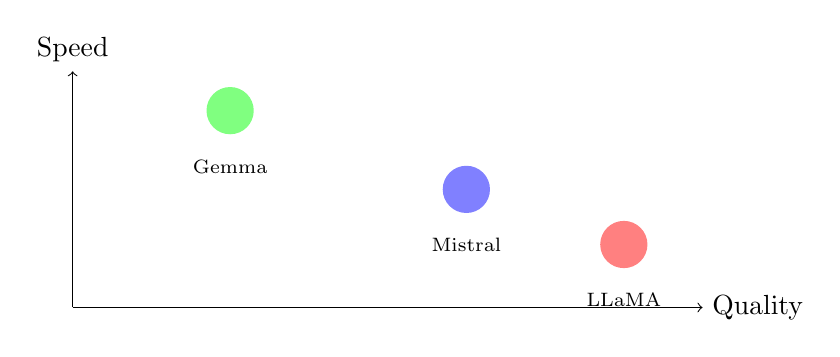
\begin{tikzpicture}
    \draw[->] (0,0) -- (8,0) node[right] {Quality};
    \draw[->] (0,0) -- (0,3) node[above] {Speed};

    \node[circle, fill=green!50, minimum size=0.6cm] at (2,2.5) {};
    \node[below] at (2,2) {\scriptsize Gemma};

    \node[circle, fill=blue!50, minimum size=0.6cm] at (5,1.5) {};
    \node[below] at (5,1) {\scriptsize Mistral};

    \node[circle, fill=red!50, minimum size=0.6cm] at (7,0.8) {};
    \node[below] at (7,0.3) {\scriptsize LLaMA};
\end{tikzpicture}
\end{center}
\end{frame}

%==============================================================================
% SECTION 6: ERROR ANALYSIS & IMPROVEMENTS
%==============================================================================
\section{Error Analysis \& Improvements}

\begin{frame}{Error Analysis \& Improvements}
\begin{columns}
\begin{column}{0.5\textwidth}
\textbf{Identified Issues:}
\begin{enumerate}
    \item \textbf{Entity Extraction}
    \begin{itemize}
        \scriptsize
        \item Hotel names with special chars missed
        \item Age group detection inconsistent
    \end{itemize}

    \item \textbf{Intent Classification}
    \begin{itemize}
        \scriptsize
        \item Confusion between search/recommendation
        \item Multi-intent queries not handled
    \end{itemize}

    \item \textbf{Graph Retrieval}
    \begin{itemize}
        \scriptsize
        \item Empty results for rare cities
        \item Slow for complex traversals
    \end{itemize}
\end{enumerate}
\end{column}

\begin{column}{0.5\textwidth}
\textbf{Improvements Made:}
\begin{enumerate}
    \item \textbf{Entity Extraction}
    \begin{itemize}
        \scriptsize
        \item Added rating keywords (cleanliness, comfort)
        \item Expanded traveller type vocabulary
    \end{itemize}

    \item \textbf{Intent Classification}
    \begin{itemize}
        \scriptsize
        \item Increased training data per class
        \item Added confidence threshold
    \end{itemize}

    \item \textbf{Embedding Retrieval}
    \begin{itemize}
        \scriptsize
        \item Dual approach (Node2Vec + Text)
        \item FAISS for fast similarity search
    \end{itemize}
\end{enumerate}
\end{column}
\end{columns}

\vspace{0.3cm}
\textbf{Future Work:} Multi-intent support, caching layer, conversation memory
\end{frame}

%==============================================================================
% SECTION 7: LIVE DEMO
%==============================================================================
\section{Live Demo}

\begin{frame}{Pipeline Recap for Demo}
\begin{center}
\begin{tikzpicture}[node distance=0.8cm, scale=0.75, transform shape,
    step/.style={rectangle, draw, fill=blue!20, text width=3cm, text centered, minimum height=0.7cm, rounded corners}]

    \node[step, fill=green!30] (s1) {1. User Query};
    \node[step, right=of s1] (s2) {2. BERT Intent};
    \node[step, right=of s2] (s3) {3. spaCy Entities};
    \node[step, right=of s3] (s4) {4. Query Embed};

    \node[step, below=0.8cm of s1, fill=orange!30] (s5) {5. Cypher Select};
    \node[step, right=of s5, fill=orange!30] (s6) {6. Neo4j Query};
    \node[step, right=of s6, fill=purple!30] (s7) {7. FAISS Search};
    \node[step, right=of s7, fill=yellow!30] (s8) {8. Context Build};

    \node[step, below=0.8cm of s5, fill=red!30] (s9) {9. LLM Generate};
    \node[step, right=of s9, fill=green!30] (s10) {10. Response};

    \draw[->, thick] (s1) -- (s2);
    \draw[->, thick] (s2) -- (s3);
    \draw[->, thick] (s3) -- (s4);
    \draw[->, thick] (s4) -- (s5);
    \draw[->, thick] (s5) -- (s6);
    \draw[->, thick] (s6) -- (s7);
    \draw[->, thick] (s7) -- (s8);
    \draw[->, thick] (s8) -- (s9);
    \draw[->, thick] (s9) -- (s10);

\end{tikzpicture}
\end{center}

\vspace{0.3cm}
\textbf{Demo Features:}
\begin{itemize}
    \item Switch between embedding models (Node2Vec / Text)
    \item Switch between LLMs (Gemma / Mistral / LLaMA)
    \item Real-time pipeline visualization
    \item Streamlit UI showing each processing step
\end{itemize}
\end{frame}

%------------------------------------------------------------------------------
\begin{frame}{Demo Queries}
\textbf{Test Queries for Live Demo:}

\begin{enumerate}
    \item \textbf{Recommendation:} ``Recommend me a good hotel in Tokyo''

    \item \textbf{Traveller Preference:} ``Best hotels for solo female travelers''

    \item \textbf{Visa Query:} ``Do I need a visa to travel from India to Dubai?''

    \item \textbf{Rating Filter:} ``Hotels with cleanliness rating above 9''

    \item \textbf{Comparison:} ``Compare The Azure Tower and Marina Bay''

    \item \textbf{Complex:} ``Find comfortable business hotels in Paris for travelers aged 25-34''
\end{enumerate}

\vspace{0.3cm}
\begin{center}
\textbf{[LIVE DEMO]}
\end{center}
\end{frame}

%==============================================================================
\begin{frame}
\begin{center}
\Huge Thank You!

\vspace{1cm}
\Large Questions?
\end{center}
\end{frame}

\end{document}
